\documentclass[journal]{IEEEtran}

\usepackage{ifpdf}

\usepackage{cite}

\ifCLASSINFOpdf
  \usepackage[pdftex]{graphicx}
  % declare the path(s) where your graphic files are
  \graphicspath{{images}}
  % and their extensions so you won't have to specify these with
  % every instance of \includegraphics
  \DeclareGraphicsExtensions{.pdf,.jpeg,.png}
\else
  % or other class option (dvipsone, dvipdf, if not using dvips). graphicx
  % will default to the driver specified in the system graphics.cfg if no
  % driver is specified.
  \usepackage[dvips]{graphicx}
  % declare the path(s) where your graphic files are
  \graphicspath{images}
  % and their extensions so you won't have to specify these with
  % every instance of \includegraphics
  \DeclareGraphicsExtensions{.eps}
\fi

\usepackage[cmex10]{amsmath}
\usepackage{amsfonts}
\usepackage{amssymb}


\usepackage{algorithmic}

\usepackage{array}
\ifCLASSOPTIONcompsoc
  \usepackage[caption=false,font=normalsize,labelfont=sf,textfont=sf]{subfig}
\else
  \usepackage[caption=false,font=footnotesize]{subfig}
\fi

\usepackage{fixltx2e}

\usepackage{stfloats}

\ifCLASSOPTIONcaptionsoff
  \usepackage[nomarkers]{endfloat}
 \let\MYoriglatexcaption\caption
 \renewcommand{\caption}[2][\relax]{\MYoriglatexcaption[#2]{#2}}
\fi

\usepackage{url}

% correct bad hyphenation here
\hyphenation{op-tical net-works semi-conduc-tor}

\begin{document}

\title{FollowBot Android Application}


\author{Arian~Stolwijk,~\IEEEmembership{4001079}
        and Radu~Florea,~\IEEEmembership{4330358}}% <-this % stops a space

% The paper headers
\markboth{IN4254 - Smart Phone Sensing}%
{}
% make the title area
\maketitle

% As a general rule, do not put math, special symbols or citations
% in the abstract or keywords.
\begin{abstract}
The abstract goes here.
\end{abstract}

\section{Introduction}
% The very first letter is a 2 line initial drop letter followed
% by the rest of the first word in caps.
%
% form to use if the first word consists of a single letter:
% \IEEEPARstart{A}{demo} file is ....
%
% form to use if you need the single drop letter followed by
% normal text (unknown if ever used by IEEE):
% \IEEEPARstart{A}{}demo file is ....
%
% Some journals put the first two words in caps:
% \IEEEPARstart{T}{his demo} file is ....
%
% Here we have the typical use of a "T" for an initial drop letter
% and "HIS" in caps to complete the first word.
\IEEEPARstart{T}{his} demo file is intended to serve as a ``starter file''
for IEEE journal papers produced under \LaTeX\ using
IEEEtran.cls version 1.8 and later.
% You must have at least 2 lines in the paragraph with the drop letter
% (should never be an issue)
I wish you the best of success.

\section{Robot Detection}
In order to control the robot, it must be first detected and paired with the Android Smart Phone. Since pairing between the phone and the robot is achieved by simply connecting to the \texttt{IOIO} board's Bluetooth module, only the detection of the robot needs to be considered. Furthermore, accurate estimates of the robot's distance and orientation with respect to the user are needed so that a good control can be achieved.

\subsection{Shape Recognition}
One straightforward solution to the detection problem is to simply make use of the phone's camera for detecting and tracking three colored spherical objects that are placed on the top of the robot.

We first start off by converting the colored image from the standard RGB geometry into the HSV (Hue-Saturation-Value) representation. This is done due to the fact that it is much easier to filter out a range of colors in the HSV representation than in the normal RGB case. The HSV color cylinder is presented in Figure \ref{fig:sim}.
\begin{figure}[!htpb]
\centering
\includegraphics[width=2in]{images/hsv_representation}
\caption{Hue-Saturation-Value color cylinder}
\label{fig:sim}
\end{figure}

Using this representation, the images from the phone's camera can be thresholded based on the colors they contain. Since we are interested in detecting blue and green objects, a set of minimum and maximum bounds has been defined for each of the colors.

The thresholding procedure results in two different images, i.e. one containing data for the color blue and the other one for the color green. These two images are combined into one through the use of an \texttt{OR} operation. This process is shown in Figure \ref{fig:thresh}.
\begin{figure}[!htpb]
\centering
%\includegraphics[width=2in]{figures/hsv_representation}
\caption{Image thresholding process}
\label{fig:thresh}
\end{figure}

Having the thresholded image obtained, the Circle Hough Transform (CHT) can be applied in order to obtain the three circles present in the image, and track them.

The basic idea underlying the Hough Transform is that, given an image containing a circle described as:
\begin{equation}
\left(x-a\right)^2 + \left(y-b\right)^2 = r^2
\end{equation}
where $(a,b)$ are the coordinates of the circle's center and $r$ is its radius, an arbitrary edge point $(x_i, y_i)$ will be transformed into a right circular cone in the $(a,b,r)$ parameter space. If the image points lie in a circle, then the cones will intersect at a single point in $(a,b,r)$, corresponding to the parameters of the circle [CITE HERE!].

The CHT is also capable of finding circles that are partially hidden, if enough of their boundary is visible. This feature is especially important for the project, since the lighting conditions are not perfect, resulting in parts of the tracking balls that will not be contained in the thresholded image. Such a case is presented in Figure \ref{fig:cht}.
\begin{figure}[!htpb]
\centering
%\includegraphics[width=2in]{figures/hsv_representation}
\caption{Circle detection using Hough Transform. Left: Thresholded image, with detected circles. Right: RGB image (in imperfect lighting conditions), with detected circles}
\label{fig:cht}
\end{figure}

As it can be observed, the Hough Transform achieves circle detection even if the image does not contain the entire shape.

The presented detection method has been implemented, with the help of the \texttt{OpenCV} library, in \texttt{C++}, and it was imported in the Android application through the \texttt{JNI} (Java Native Interface).

\subsection{Distance Estimation}
In order to obtain a decently accurate distance estimation between the robot and the user, and at the same time keep the development costs low, we have explored two techniques for distance estimation, namely: estimating distance with the help of the integrated camera of the Android phone, and distance estimation using the Bluetooth RSS signal.

\subsubsection{Android Phone Camera}
The idea to use the integrated phone camera has been considered due to already having a working spherical object tracking algorithm, thus, we would only have to extend this algorithm to incorporate distance estimation.

From a geometrical point of view, the user to robot distance estimation is presented in Figure \ref{fig:dist_camera}.
\begin{figure}[!htpb]
\centering
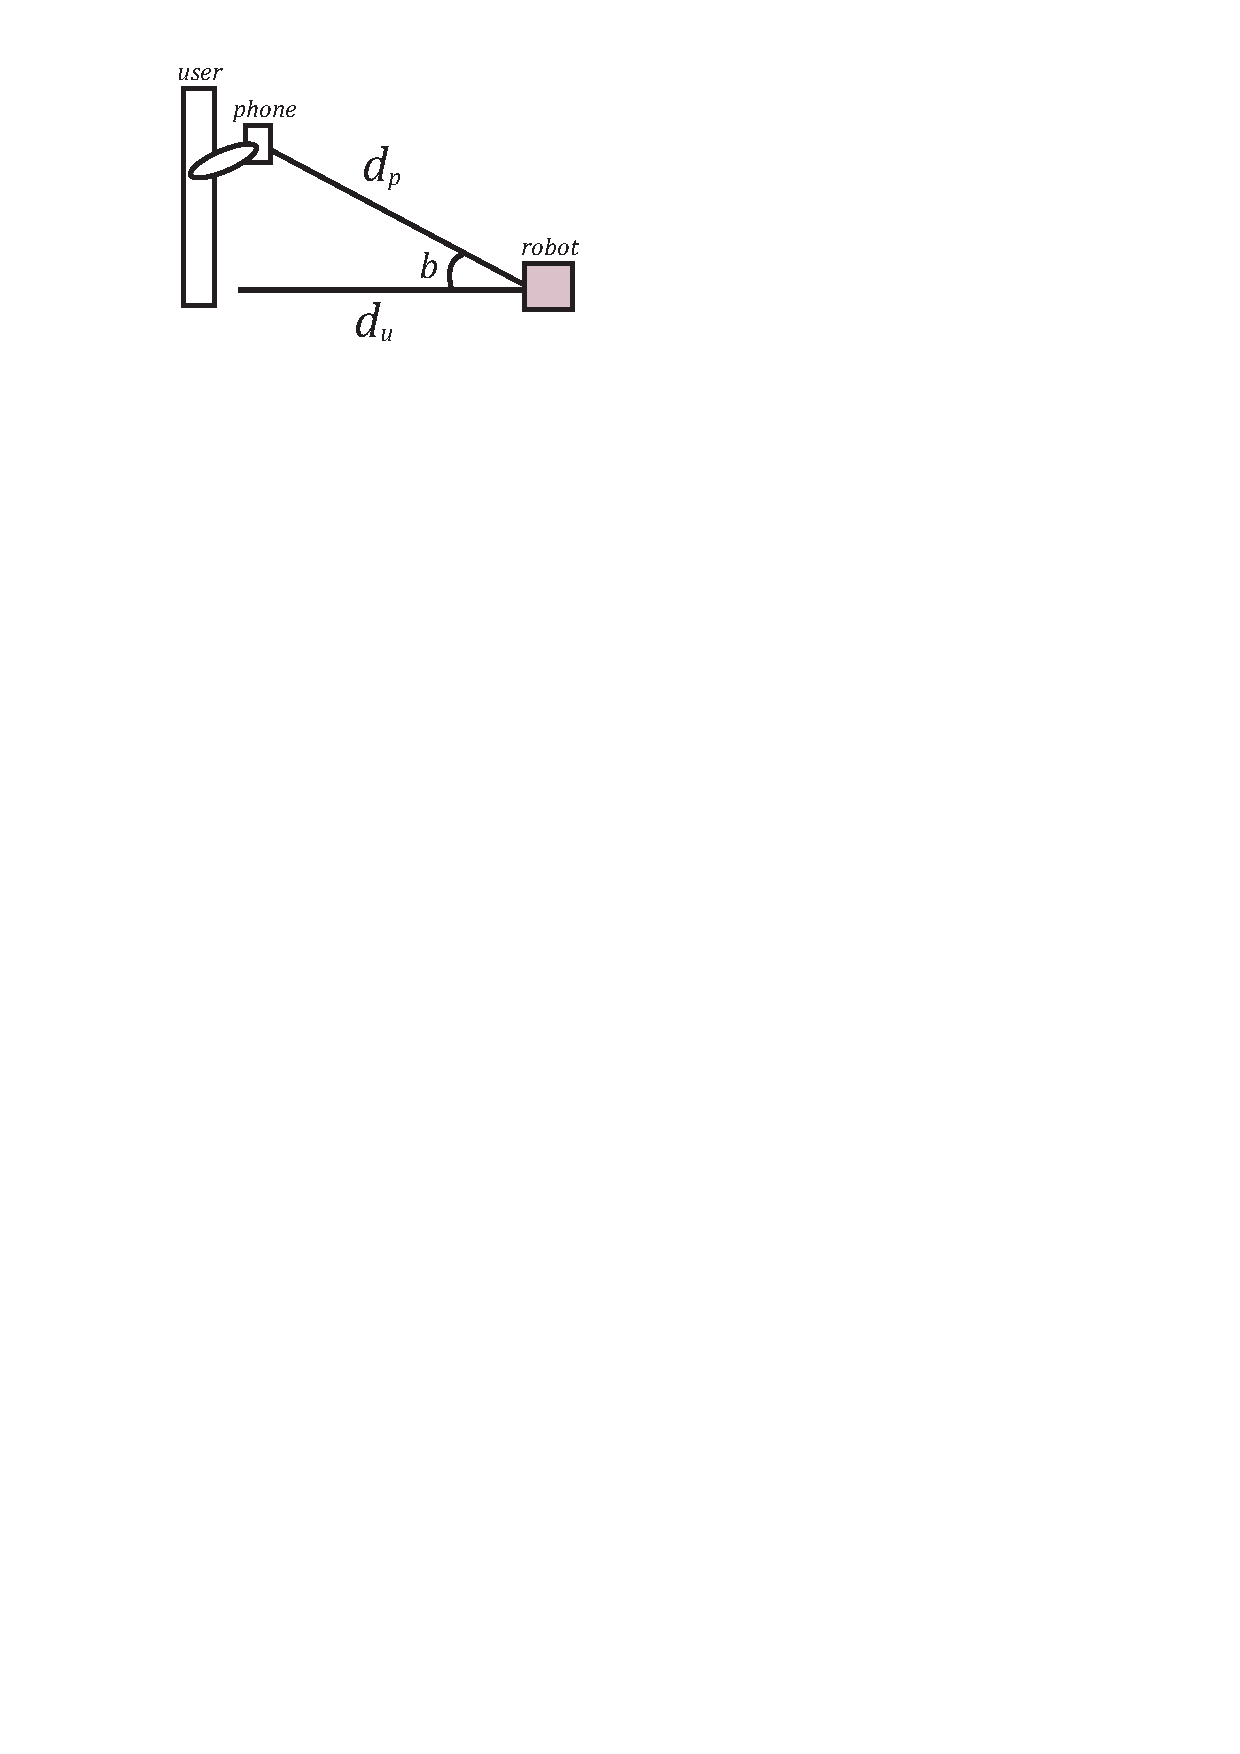
\includegraphics[width=2in]{images/distance_meas}
\caption{Side-view of the distance estimation, using the phone camera. Phone-robot distance is represented by $d_p$, user-robot distance is represented by $d_u$, and the skew angle is represented by $b$}
\label{fig:dist_camera}
\end{figure}

It can be observed that the user-robot distance $d_u$ can be obtained by simply applying the following formula:
\begin{equation}
d_u=d_pcos(b)
\end{equation}
where the phone-robot distance and the skew angle estimates are given by $d_p$ and $b$, respectively.

In order to obtain an estimate of $d_p$, the radius values of the closest circle (i.e. the largest radius $r_{max})$ has been taken at different distance points, after which a linear interpolation has been applied to these data points, resulting in the following equation for the phone-robot distance estimate
\begin{equation}
d_p=-\frac{24}{31}r_{max}+\frac{1995}{31}
\end{equation}

The skew angle $b$ is estimated in a similar fashion. Considering that the tracking balls are placed in an equilateral triangle shape, a skew angle of $90^{\circ}$ (phone is directly above the robot) corresponds to reading an angle of $60^{\circ}$ from the triangle determined by the tracking objects. Furthermore, when the skew angle decreases, by always taking the largest angle of the triangle

\subsubsection{Bluetooth RSS Signal}

\subsection{Orientation Estimation}
\begin{figure}[!htpb]
\centering
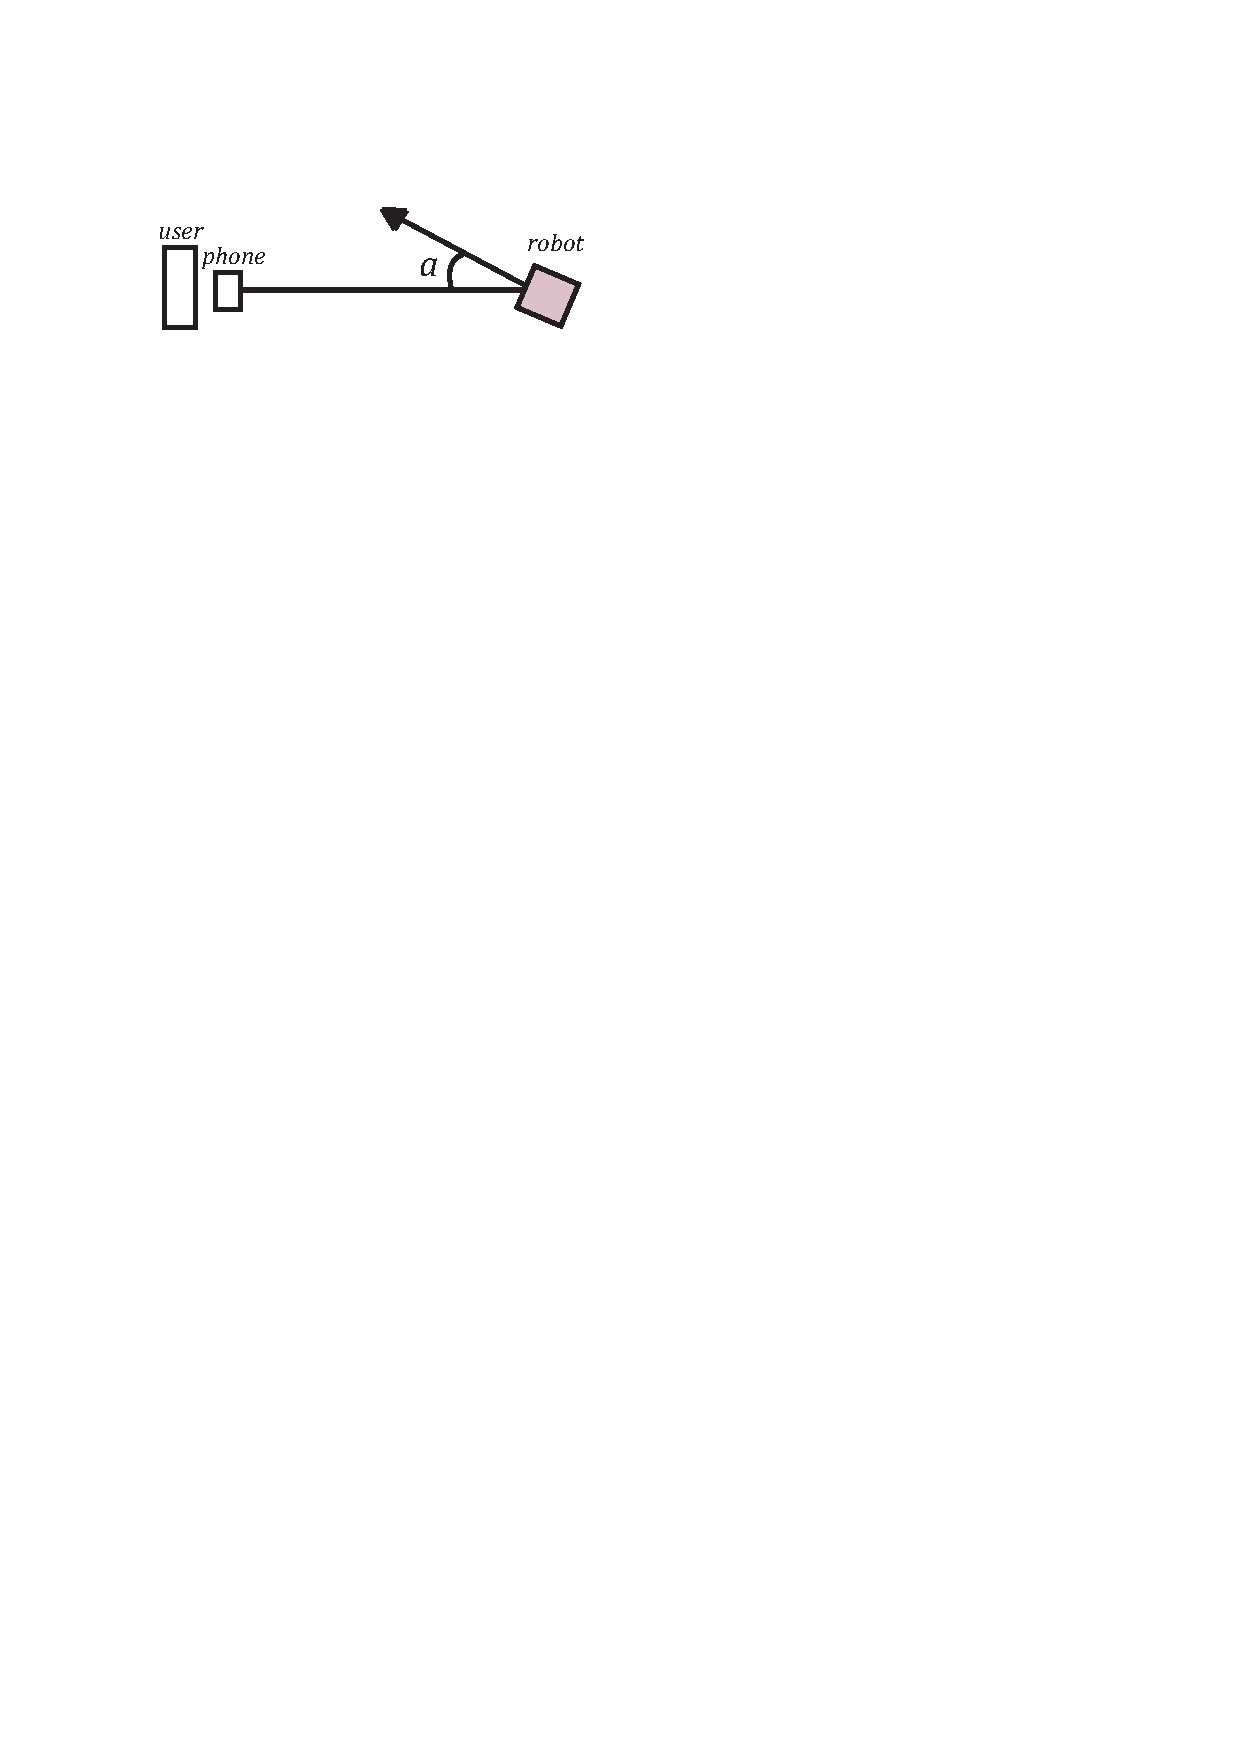
\includegraphics[width=2in]{images/orientation_meas}
\caption{Top-view of the orientation estimation, using the phone camera}
\label{fig:orient_camera}
\end{figure}

\subsubsection{Subsubsection Heading Here}
Subsubsection text here.


% An example of a floating figure using the graphicx package.
% Note that \label must occur AFTER (or within) \caption.
% For figures, \caption should occur after the \includegraphics.
% Note that IEEEtran v1.7 and later has special internal code that
% is designed to preserve the operation of \label within \caption
% even when the captionsoff option is in effect. However, because
% of issues like this, it may be the safest practice to put all your
% \label just after \caption rather than within \caption{}.
%
% Reminder: the "draftcls" or "draftclsnofoot", not "draft", class
% option should be used if it is desired that the figures are to be
% displayed while in draft mode.
%
%\begin{figure}[!t]
%\centering
%\includegraphics[width=2.5in]{myfigure}
% where an .eps filename suffix will be assumed under latex,
% and a .pdf suffix will be assumed for pdflatex; or what has been declared
% via \DeclareGraphicsExtensions.
%\caption{Simulation Results.}
%\label{fig_sim}
%\end{figure}

% Note that IEEE typically puts floats only at the top, even when this
% results in a large percentage of a column being occupied by floats.


% An example of a double column floating figure using two subfigures.
% (The subfig.sty package must be loaded for this to work.)
% The subfigure \label commands are set within each subfloat command,
% and the \label for the overall figure must come after \caption.
% \hfil is used as a separator to get equal spacing.
% Watch out that the combined width of all the subfigures on a
% line do not exceed the text width or a line break will occur.
%
%\begin{figure*}[!t]
%\centering
%\subfloat[Case I]{\includegraphics[width=2.5in]{box}%
%\label{fig_first_case}}
%\hfil
%\subfloat[Case II]{\includegraphics[width=2.5in]{box}%
%\label{fig_second_case}}
%\caption{Simulation results.}
%\label{fig_sim}
%\end{figure*}
%
% Note that often IEEE papers with subfigures do not employ subfigure
% captions (using the optional argument to \subfloat[]), but instead will
% reference/describe all of them (a), (b), etc., within the main caption.


% An example of a floating table. Note that, for IEEE style tables, the
% \caption command should come BEFORE the table. Table text will default to
% \footnotesize as IEEE normally uses this smaller font for tables.
% The \label must come after \caption as always.
%
%\begin{table}[!t]
%% increase table row spacing, adjust to taste
%\renewcommand{\arraystretch}{1.3}
% if using array.sty, it might be a good idea to tweak the value of
% \extrarowheight as needed to properly center the text within the cells
%\caption{An Example of a Table}
%\label{table_example}
%\centering
%% Some packages, such as MDW tools, offer better commands for making tables
%% than the plain LaTeX2e tabular which is used here.
%\begin{tabular}{|c||c|}
%\hline
%One & Two\\
%\hline
%Three & Four\\
%\hline
%\end{tabular}
%\end{table}


% Note that IEEE does not put floats in the very first column - or typically
% anywhere on the first page for that matter. Also, in-text middle ("here")
% positioning is not used. Most IEEE journals use top floats exclusively.
% Note that, LaTeX2e, unlike IEEE journals, places footnotes above bottom
% floats. This can be corrected via the \fnbelowfloat command of the
% stfloats package.

\section{Activity Monitoring}

When the user moves the particle filter should be updated. To know when the
user is moving can be done with Activity Monitoring. Activity monitoring uses
sensors to identify what the user is doing, for example standing, walking,
cycling or running. Using the activity a speed can be associated to update the
particles in the particle filter. For our application differentiating between
standing still and walking will be enough. \cite{ravi2005activity} showed
different classification techniques using an accelerometer. Features they use
are the mean, standard deviation, energy, correlation and periodicity.  For the
two different activities we expected that the energy and the periodicity to
be enough. \cite{ravi2005activity} also compares different classifiers.
Although the $k$-Nearest-Neighbors is not the best, it is really close to the
best classifier. This combined with that it is relatively easy to implement
makes the kNN classifier a good choice.

The accelerometer stores the $x$, $y$ and $z$ acceleration in a fixed size
data structure with a size of 128 values. This corresponds with a window size
of approximately $1.3$ seconds.

The feature vector $\mathbf{v} = [ZC(\vec x) / t, P(\vec x)/ n]^\intercal$,
where $t$ is the time between the first and last points, and $ZC(\vec x)$ and
$P(\vec x)$ are calculated by:

\[
  s(x,y) = \left\{
    \begin{array}{l l}
      1 & \quad \text{if~} x y < 0 \\
      0 & \quad \text{if~} x y >= 0
  \end{array} \right.
\]

\[
  ZC(\vec x) = \sum^{n-1}_{i=0} s(x_i, x_{i+1})
\]

\[
  P = \sum^{n}_{i=0} x_i^2
\]

The kNN classifier consists out of two phases: a learning phase, where feature
vectors with a known class (activity in this case) are stored. This results in
in a plot like figure~\ref{fig:knn-data}.

\begin{figure}
  \centering
  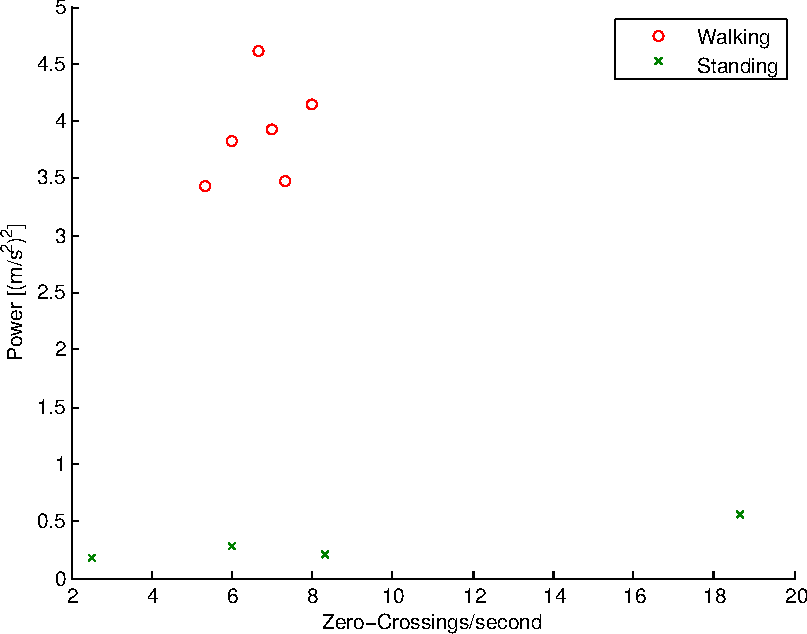
\includegraphics[width=3in]{images/knn-data.pdf}
  \caption{kNN Learning data}
  \label{fig:knn-data}
\end{figure}

The second phase is the classification phase. A newly measured feature vector
is compared with the learning data. By selecting the $n$ nearest neighbors,
counting how many points each class has and finally selecting the class with
the highest count.

The distance between a measurement and the learning data is calculated by the
Euclidean distance. Because the elements from the feature vectors have
different units, we cannot simply apply $\sqrt{ x^2+y^2 }$. Instead we need to
scale the values and make them dimensionless. We do this by finding the minimum
and maximum values of each $i$th element of all vectors, and scale the elements
between $0$ and $1$. The measured value is scaled so eventually we can
calculate the distance.

We have found that 10 learning data points, $n=3$, a window size of $1.3$s
and the chosen features give accurate results classifying walking and standing.

\section{Conclusion}
The conclusion goes here.





% if have a single appendix:
%\appendix[Proof of the Zonklar Equations]
% or
%\appendix  % for no appendix heading
% do not use \section anymore after \appendix, only \section*
% is possibly needed

% use appendices with more than one appendix
% then use \section to start each appendix
% you must declare a \section before using any
% \subsection or using \label (\appendices by itself
% starts a section numbered zero.)
%


\appendices
\section{Appendix}


% Can use something like this to put references on a page
% by themselves when using endfloat and the captionsoff option.
\ifCLASSOPTIONcaptionsoff
  \newpage
\fi



% trigger a \newpage just before the given reference
% number - used to balance the columns on the last page
% adjust value as needed - may need to be readjusted if
% the document is modified later
%\IEEEtriggeratref{8}
% The "triggered" command can be changed if desired:
%\IEEEtriggercmd{\enlargethispage{-5in}}

% references section

% can use a bibliography generated by BibTeX as a .bbl file
% BibTeX documentation can be easily obtained at:
% http://www.ctan.org/tex-archive/biblio/bibtex/contrib/doc/
% The IEEEtran BibTeX style support page is at:
% http://www.michaelshell.org/tex/ieeetran/bibtex/
%\bibliographystyle{IEEEtran}
% argument is your BibTeX string definitions and bibliography database(s)
%\bibliography{IEEEabrv, biblio}
%
% <OR> manually copy in the resultant .bbl file
% set second argument of \begin to the number of references
% (used to reserve space for the reference number labels box)
\begin{thebibliography}{1}

\bibitem{IEEEhowto:kopka}
H.~Kopka and P.~W. Daly, \emph{A Guide to \LaTeX}, 3rd~ed.\hskip 1em plus
  0.5em minus 0.4em\relax Harlow, England: Addison-Wesley, 1999.

\end{thebibliography}

\end{document}
